\section{Introduction} \label{sec:introduction}

Agent-Based Modeling (ABM) has gained increasing adoption as a method to answer basic science questions and inform policy decisions.
Despite a wide berth of application domains --- spanning sectors like spanning transportation infrastructure, public health, telecommunications, materials science and more --- much ABM work is unified by a common theme of interest in cross-scale dynamics.
To provide such insight, ABM require sufficient scale to capture systems' emergent behaviors.
Advances in high-performance computing (HPC) have already yielded paradigm-shifting improvements to the capabilities of ABM.
However, across domains key questions still remain out of computational reach.

\begin{figure}[htbp]
\centering
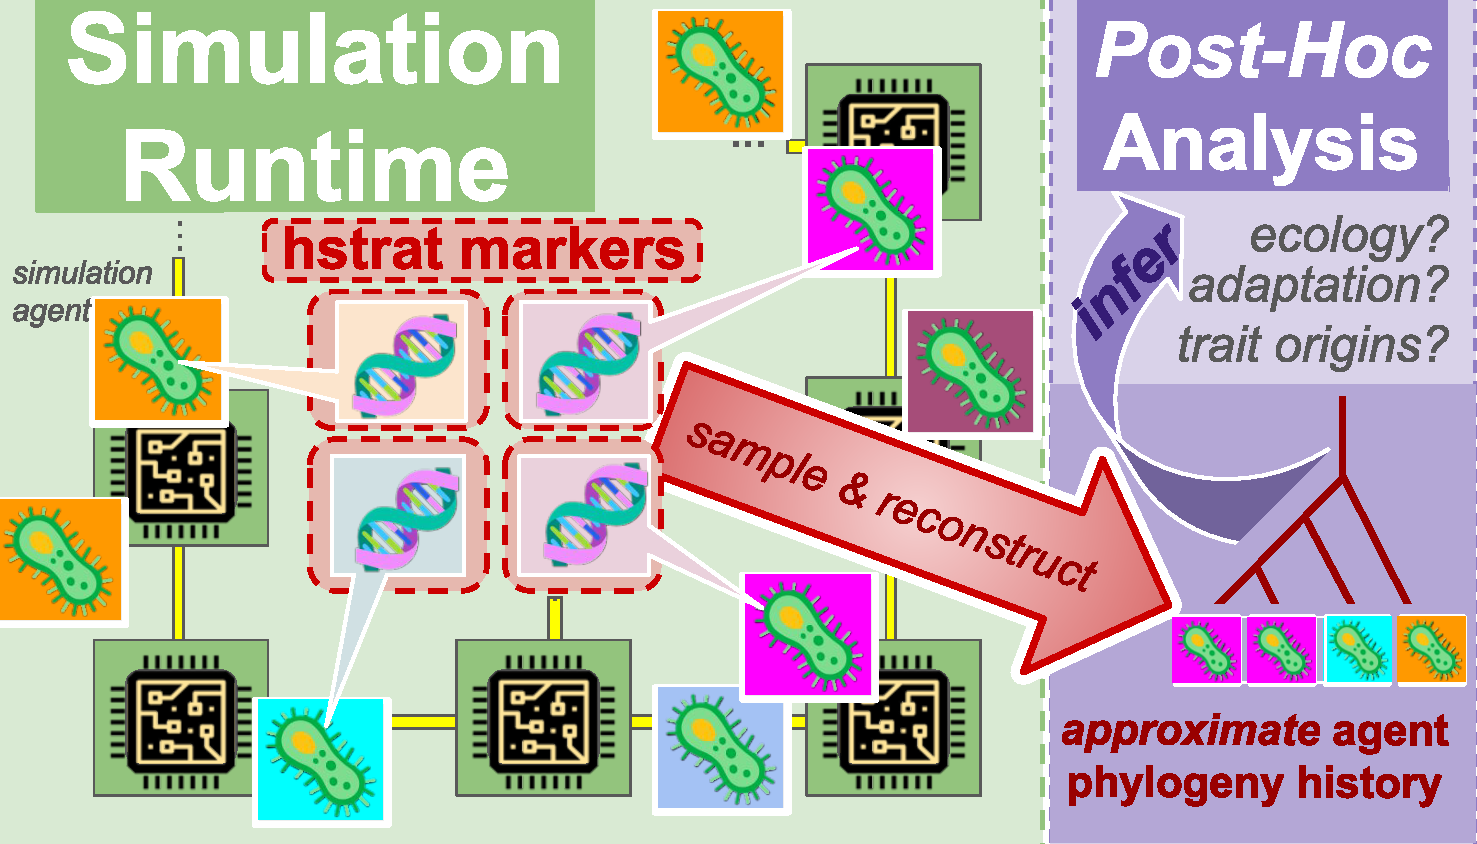
\includegraphics[width=4in]{img/runtime-posthoc-schematic.pdf}
\caption{Proposed agent-based evolutionary simulation and observation framework, using HStrat markers to estimate phylogenetic history, thereby, infer evolutionary dynamics.}
\label{fig:runtime-posthoc-schematic}
\end{figure}
Significant untapped potential for ABM scale-up has been identified in hardware-accelerator-enabled computation.
Rapid advances in the capability of accelerator devices, driven in particular by market demand for deep learning operations, is anticipated to play a key role in future advances in ABM capabilities \citep{perumalla2022computer}.
Within this category, the emerging class of fabric-based accelerators, most notably the recently-introduced 850,000 core Cerebras CS-2 Wafer Scale Engine (WSE) \citep{lauterbach2021path,lie2022cerebras}, is a particularly exciting --- and fairly uncharted, with applications to HPC workloads still in early days.
This paradigm interfaces multitudinous processor elements (PEs) in a physical lattice, with PEs executing independently using individual on-chip memory and local PEs interacting through a network-like interface.

\subsection{Objectives}

This proposal establishes foundation for next-generation accelerator-enabled ABM computation by  decentralized, approximate data export  agent-based evolutionary simulation.
In particular, we will evaluate asynchronous approaches for ABM migration/interaction on the WSE architecture to power agent-based evolution simulations, incorporating cutting-edge methods for distributed approximate phylogenetic (i.e., ancestry tree) tracking.

Proposed work advances two technical objectives:
\begin{enumerate}
\item to evaluate and demonstrate new approaches for phylogenetic tracking in a massively-distributed, resource-constrained setting,
\item to test the scalability of desynchronized agent migration procedures on WSE hardware,
\end{enumerate}

These technical capabilities will unlock capability to investigate a broad array of science questions.
In this proposal, we focus on one science objective:
\begin{enumerate}
\item to evaluate how phylogenetic structure scales across orders-of-magnitude population sizes, and the extent to which commonly used phylogeny structure metrics are scale-invariant or scale-sensitive.
\end{enumerate}

Proposed work falls within the domain of agent-based evolution modeling, and uses it to explores phylogenetics-related inquiry by leveraging Cerebras WSE hardware.
Our dual technical objectives constitute significant advancement of methodological capabilities within digital evolution, and our project will directly address fundamental open questions within the domain of phylogenetic theory.
However, findings and methodologies will also generalize to other ABM domains beyond evolutionary simulation and to broader classes of highly-distributed HPC architectures.

\subsection{Agent-based Evolution Simulation}

Evolutionary processes do not confine to matters of natural history.
Rather, evolutionary processes pervade our contemporary, everyday world.
Key societal challenges root in evolving systems: antibiotic resistance, epidemiology, conservation biology, and oncology among others.  % citations?
Evolutionary biology provides the fundamental foothold to efforts to address these problems \citep{aktipis2013evolutionary}.

Mathematical and computational modeling complements natural history field work and benchtop evolution experiments as a crucial third leg to stand evolutionary inquiry.
Simulation-based approaches provide key capabilities complementary to work with natural systems: complete observability, arbitrary manipulability, and rapid generational turnover.
Within this context, agent-based simulation plays an important connective role between natural systems and abstracted, aggregate-based mathematical and numerical models.
Agent-based approaches instantiate \textit{bona fide} evolutionary processes that track populations of virtual genomes subject to mutation, heredity, and selection \citep{pennock2007models}.
This characteristic incorporates some of the critical complications and subtleties characteristic of natural systems --- e.g., arbitrary agent behavior, sophisticated agent-agent interactions, complex genotype-phenotype maps, albeit at significantly reduced scope and sophistication.

Indeed, agent-based evolution approaches have provided means for fruitful investigation of wide-ranging hypotheses, including evolution of evolvability \citep{wilke2001evolution}, host-parasite co-evolution \citep{zaman2014coevolution}, evolution of complex traits \citep{lenski2003evolutionary}.

Ambitious work advancing the field increasingly targets large cross-scale questions, including major transitions in evolution (e.g., multicellularity and symbiosis) \citep{goldsby2020major,vostinar2021symbiosis} and open-ended evolution (e.g., long-term trajectories of complex ecosystems with strong biotic selection) \citep{stanley2019open,taylor2016open}.
Progress on these fronts demands computational substrate for orders-of-magnitude larger simulation scale than tractable today \citep{moreno2022exploring,channon2019maximum}.

%as well as scenarios where replicating entities like cultural artifacts or computer viruses.
% At the frontiers of evolutionary computation, there is in particular growing interest in the question of ``open-ended evolution'' \citep{}.
% This refers to the problem of the inability to recreate the ongoing generation of novelty, complexity, and adaptation within the natural world.

\subsection{HPC and Agent-based Evolution}
% opportunity


% Evolutionary questions often explicitly span scopes, with key areas of inquiry including ecologies of interacting populations and assembly of individuals into multicellular organisms and eusocial colonies \citep{morenoDISHTINYTODO, citephageTODO}.
Researchers using agent-based evolution recognize HPC as critical to the future of the field \citep{ackley2016indefinite}.
Indeed, the field has played host to notable boundary-pushing approaches to computing at the frontiers of computing hardware and modalities such as best-effort computing, reservoir computing, global-scale time-available computing, and modular tile-based computing in addition to more traditional cluster and GPU-oriented approaches \citep{moreno2021conduit,ackley2020best,ackley2023robust,heinemann2008artificial,miikkulainen2024evolving}.
The diversity and, in cases, novelty of HPC within evolutionary simulation stems in large part from unique properties largely distinct from other HPC application domains.

Given its inherent underlying stochastic nature and the stabilizing influence of adaptive selection, evolutionary simulation can often tolerate significant arbitrary asynchronicity or even entirely lost simulation components (e.g., dropped messages, crashed nodes, etc.).
Likewise, digital evolution is typically amenable to locality restrictions of computation due to the inherent spatial structure of natural systems we are seeking to model.
% In particular, massively-distributed, spatial computing being directly highlighted to be of particular interest \citep{ackleyTODO}.
Because agent behavior evolves over time, the influence of population-level drift and adaptive change can inject extreme heterogeneity to the computational workload profile of evolutionary simulation over time and simulation space.
Finally, emerging directions have begun to tilt implementation towards more challenging communication-intensive qualities.
The largely-decoupled nature of classic approaches within evolutionary computation like island models or controller/worker schemes  \citep{bennett1999building,cantu2001master} no longer suffice to realize the dynamic, communication-intensive interaction characteristic of major transitions and open-ended evolution \citep{moreno2022engineering}.

These distinctive properties, position agent-based evolution as a potentially valuable testbed for HPC innovation and leadership.
There is reason to expect a highly synergistic, reciprocal relationship between digital evolution and the broader HPC enterprise.
Work proposed here steps in this direction, seeking to blaze new territory that opens new possibilities to benefit broader constituencies of ABM/HPC practitioners.

However, despite the strong motivation for large-scale simulation, the algorithmic pliability of evolutionary simulation, and the increasing availability of highly-capable parallel, distributed, and accelerator-driven hardware platforms, significant methodological limitations currently hold back progress achieving widespread scale-up the field of digital evolution.
Through work proposed here, we will take significant steps to resolving this knot and thereby position the field to benefit significantly from this emerging class of hardware accelerators.

\subsection{Phylogenetic Tracking Methods}

To serve as a useful experimental platform, digital evolution simulations must be observable.
In addition to end-state information (i.e., evolved traits), scientific questions demand information sufficient to characterize underlying mode and tempo of evolution.
Additionally, it is often useful to be able to trace the history of notable evolutionary events (e.g., extinctions, evolutionary innovations)
Observability counts, too, in application-oriented aspects of evolutionary computation, where such data serves as a critical diagnostic to tune configuration for good performance \citep{hernandez2022can}.

In evolutionary biology, phylogenetic history is a valuable tool to triangulating the context of notable evolutionary events, as well as characterizing the underlying mode and tempo of evolution.
The same holds true in evolutionary simulation.
% https://github.com/mmore500/phylotrack-algorithm-analysis/blob/fe16d2b2d7df99faade09c01b72f681160749f51/tex/text/body/introduction.tex
In addition to addressing questions of natural history, access to the phylogenetic record of biological life has proven informative to conservation biology, epidemiology, medicine, and biochemistry among other domains \citep{faithConservationEvaluationPhylogenetic1992, STAMATAKIS2005phylogenetics, frenchHostPhylogenyShapes2023,kim2006discovery}.
Nonetheless, existing analyses of phylogenetic structure within digital systems have already proven valuable, enabling diagnosis of underlying evolutionary dynamics \citep{moreno2023toward,hernandez2022can,shahbandegan2022untangling, lewinsohnStatedependentEvolutionaryModels2023a} and even serving as mechanism to guide evolution in application-oriented domains \citep{lalejini2024phylogeny,lalejini2024runtime,murphy2008simple,burke2003increased}.
Further, comparison of observed phylogenies against simulation phylogenies can be used to evaluate hypotheses for underlying dynamics within real-life evolutionary/epidemiological systems \citep{giardina2017inference,voznica2022deep}.

Unfortunately, existing approaches to recording phylogenetic history from digital evolution simulations do not scale robustly.
Simulation phylogenies have typically been collected using a centralized record-keeping approach where every reproduction event is stitched together in a tree data structure to produce a complete record.
Record-keeping often involves pruning the records of extinct lineages to prevent memory bloat \citep{dolson2023phylotrack}.
Although the direct-tracking approach is well suited to serial simulation substantial limitations and runtime overhead make scaling this up to highly parallel/distributed systems --- particularly those with low memory capacity like the Cerebras WSE --- essentially untenable \citep{moreno2024analysis}.

To overcome this limitation to phylogenetic analysis within many-processor HPC contexts, we have proposed a new class of reconstruction-based approaches to phylogenetic tracking in silico \citep{moreno2022hereditary}.
These approaches require no centralized data collection during simulation runtime; instead, they use post hoc comparisons between end-state agent genomes to deduce approximate phylogenetic history --- akin to how DNA-based analyses tell how lineages of contemporary organisms relate in natural history.
Figure \ref{fig:runtime-posthoc-schematic} depicts our reconstruction-based strategy.

To achieve efficient, tractable phylogenetic reconstructions in practice, some careful consideration is required.
DNA-based is notoriously data-hungry, typically requiring on the order of thousands of genome sites, and can be significantly biased by physical/functional traits of the underlying genetic information.
These concerns motivated our recent development of HStrat, a genetic architecture explicitly designed for fast, accurate reconstruction requiring only small amounts of data.
HStrat data is designed to be attached to the underlying genomes within particular digital evolution systems as a neutral annotation.
Benchmarking experiments to evaluate HStrat performance have achieved high-quality reconstruction of phylogenetic histories for tens of thousands of fully-distributed agents using just 96 bits of tracking information per agent genome.
Details on this methodology and our proposed approach to translate it to the WSE context is provided in Section \ref{sec:methods}.

% \subsection{Outline}

% The remainder of this proposal is structured as follows
% \begin{itemize}
% \item Section \ref{sec:objectives} describes proposed work,
% \item Section \ref{sec:methods} overviews proposed methods,
% \item Section \ref{sec:preliminary-work} reviews established work on this project,
% \item Section \ref{sec:conclusion} provides concluding remarks, and
% \item Section \ref{sec:key-considerations} recaps key technical considerations highlighted in the program solicitation.
% \end{itemize}
